\section{Predictiva: estimación de interferencia con predicción de trayectorias}
\label{sec:exp_e3}
%%%%%%%%%%%%%%%%%%%%%%%%%%%%%%%%%%%%%%%%%%%%%%%%%%%%%%%%%%%%%%%%%%%%%%%%%%%%%%%%

Esta sección presenta los experimentos de validación para la \textbf{estrategia Predictiva}. La estrategia Predictiva extiende la Ruta Planificada incorporando predicción de trayectorias: en lugar de evaluar la posición actual de las personas, estima sus posiciones futuras al momento en que el robot llegará a cada punto de la ruta. El costo dinámico se calcula como el número de personas cuya posición predicha se encontrará dentro de un radio $r$ de algún punto de la ruta planificada:

\begin{equation}
    D_{\text{Pred}}(v) = \bigl|\{ p_i : \exists\, (q, t_q) \in \text{ruta\_temporal}(v),\;
    \| q - \hat{p}_i(t_q) \|_2 \leq r \}\bigr|
    \label{eq:d3}
\end{equation}

\noindent donde $\hat{p}_i(t_q)$ es la posición predicha de la persona $i$ en el instante $t_q$, estimada a partir del historial de posiciones mediante velocidad promedio:

\begin{equation}
    \hat{p}_i(t) = p_i^{\text{actual}} + \bar{v}_i \cdot t
    \label{eq:prediccion}
\end{equation}

La predicción lineal con velocidad promedio permite anticipar qué personas cruzarán la ruta futura del robot, lo que en principio reduce la frecuencia con que se seleccionan fronteras hacia zonas de alta actividad dinámica.

\subsection{Diseño de los experimentos}
\label{sec:exp_e3_diseno}

Los experimentos de validación de la estrategia Predictiva comprenden \textbf{10 casos de prueba} (TC021–TC030), correspondientes a las configuraciones house $\times$ \{0, 5, 10, 15, 20\} y office $\times$ \{0, 5, 10, 15, 20\} actores, detalladas en la Tabla~\ref{tab:casos_predictiva}. Cada caso se ejecutó con \textbf{tres réplicas independientes}; el valor representativo de la estrategia Predictiva en cada configuración es la mediana de las tres réplicas. La línea de base Greedy corresponde a los experimentos G001–G010, ejecutados una vez por configuración en las mismas condiciones (duración 1800 s, $\lambda = 5$, $\mu = 0{,}01$).

\begin{table}[htbp]
    \centering
    \caption{Casos de prueba de validación: estrategia Predictiva y Greedy. Cada caso corresponde a una combinación de entorno y número de actores.}
    \label{tab:casos_predictiva}
    \begin{tabular}{cccrr}
        \toprule
        \textbf{Caso (Predictiva)} & \textbf{Caso (Greedy)} & \textbf{Entorno} & \textbf{Actores} & \textbf{Réplicas (Predictiva)} \\
        \midrule
        TC021 & G001 & house  &  0 & V061–V063 \\
        TC022 & G002 & office &  0 & V064–V066 \\
        TC023 & G003 & house  &  5 & V067–V069 \\
        TC024 & G004 & office &  5 & V070–V072 \\
        TC025 & G005 & house  & 10 & V073–V075 \\
        TC026 & G006 & office & 10 & V076–V078 \\
        TC027 & G007 & house  & 15 & V079–V081 \\
        TC028 & G008 & office & 15 & V082–V084 \\
        TC029 & G009 & house  & 20 & V085–V087 \\
        TC030 & G010 & office & 20 & V088–V090 \\
        \bottomrule
    \end{tabular}
\end{table}

La normalización global min-máx de la Ecuación~(\ref{eq:norm}) se aplicó sobre la unión de valores de Predictiva y Greedy, con los rangos globales detallados en la Tabla~\ref{tab:rangos_globales_e3}.

\begin{table}[htbp]
    \centering
    \caption{Rangos globales de normalización para la comparación Predictiva vs Greedy.}
    \label{tab:rangos_globales_e3}
    \begin{tabular}{lrr}
        \toprule
        \textbf{Métrica} & \textbf{Mínimo} & \textbf{Máximo} \\
        \midrule
        Celdas fantasma & 0 & 153 \\
        Entropía del mapa & $9{,}42 \times 10^{-6}$ & $2{,}06 \times 10^{-4}$ \\
        Frames procesados & 98 & 648 \\
        \bottomrule
    \end{tabular}
\end{table}

\subsection{Resultados por métrica}
\label{sec:exp_e3_metricas}

La Tabla~\ref{tab:e3_ghost} y la Figura~\ref{fig:e3_ghost} presentan los resultados de celdas fantasma para cada configuración.

\begin{table}[htbp]
    \centering
    \caption{Celdas fantasma (valor final) por configuración: Predictiva vs Greedy. Valores en negrita indican la estrategia ganadora. Menor es mejor.}
    \label{tab:e3_ghost}
    \begin{tabular}{lrrr}
        \toprule
        \textbf{Configuración} & \textbf{Predictiva (mediana)} & \textbf{Greedy} & \textbf{\% dif.} \\
        \midrule
        house-0   & 30              & \textbf{15}  & $+100\%$ \\
        office-0  & 14              & \textbf{13}  & $+8\%$   \\
        house-5   & \textbf{0}      & 81           & $-100\%$ \\
        office-5  & 99              & \textbf{78}  & $+27\%$  \\
        house-10  & \textbf{0}      & 83           & $-100\%$ \\
        office-10 & \textbf{18}     & 125          & $-86\%$  \\
        house-15  & \textbf{0}      & 118          & $-100\%$ \\
        office-15 & \textbf{0}      & 153          & $-100\%$ \\
        house-20  & \textbf{0}      & 131          & $-100\%$ \\
        office-20 & \textbf{63}     & 83           & $-24\%$  \\
        \bottomrule
    \end{tabular}
\end{table}

\begin{figure}[htbp]
    \centering
    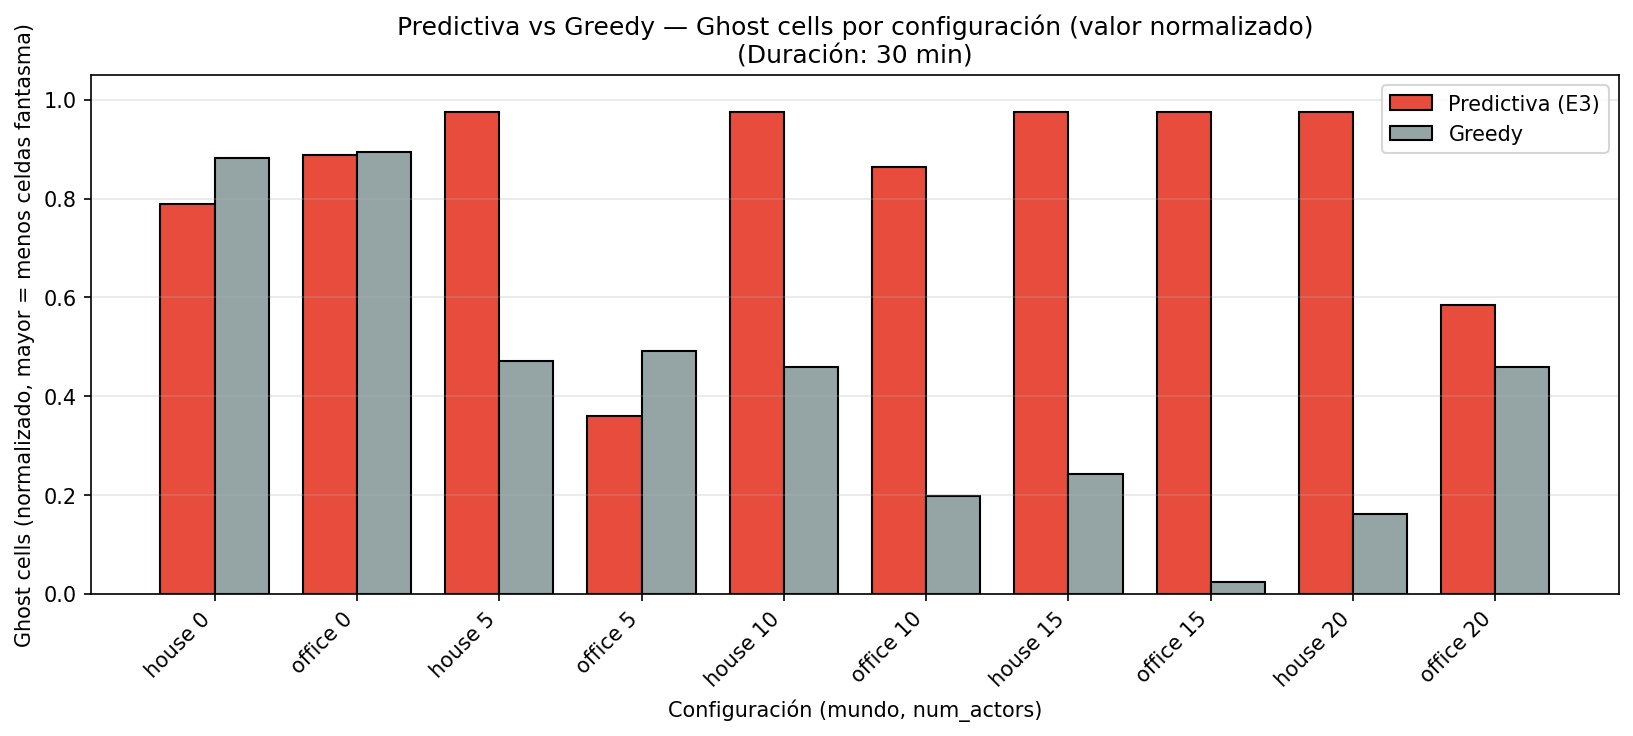
\includegraphics[width=0.85\textwidth]{figures/experiments/e3_vs_greedy_05_ghost_normalizado.png}
    \caption{Celdas fantasma normalizadas por configuración. Valor normalizado mayor indica menor número de celdas fantasma (mejor precisión del mapa). Predictiva supera a Greedy en 7 de las 10 configuraciones.}
    \label{fig:e3_ghost}
\end{figure}

La estrategia Predictiva supera a Greedy en celdas fantasma en \textbf{7 de las 10} configuraciones. Las tres excepciones corresponden a los escenarios sin actores o con densidad baja (house-0, office-0, office-5), donde la interferencia dinámica es nula o escasa y la predicción de trayectorias no aporta ventaja alguna. En el entorno house, la estrategia Predictiva logra cero celdas fantasma en todas las configuraciones con actores (house-5 a house-20). En office, la ventaja es también consistente a partir de 10 actores, aunque con magnitudes variables: una reducción del 86\% en office-10, eliminación total en office-15 y una reducción del 24\% en office-20.

La Tabla~\ref{tab:e3_entropy} y la Figura~\ref{fig:e3_entropy} presentan los resultados de entropía del mapa.

\begin{table}[htbp]
    \centering
    \caption{Entropía del mapa (valor final) por configuración: Predictiva vs Greedy. Valores en negrita indican la estrategia ganadora. Mayor es mejor.}
    \label{tab:e3_entropy}
    \begin{tabular}{lrrr}
        \toprule
        \textbf{Configuración} & \textbf{Predictiva (mediana)} & \textbf{Greedy} & \textbf{\% dif.} \\
        \midrule
        house-0   & $1{,}0 \times 10^{-5}$  & $\mathbf{1{,}3 \times 10^{-4}}$ & $-92\%$ \\
        office-0  & $1{,}1 \times 10^{-4}$  & $\mathbf{2{,}1 \times 10^{-4}}$ & $-45\%$ \\
        house-5   & $1{,}1 \times 10^{-4}$  & $\mathbf{1{,}7 \times 10^{-4}}$ & $-32\%$ \\
        office-5  & $8{,}5 \times 10^{-5}$  & $\mathbf{1{,}1 \times 10^{-4}}$ & $-20\%$ \\
        house-10  & $6{,}2 \times 10^{-5}$  & $\mathbf{6{,}6 \times 10^{-5}}$ & $-7\%$  \\
        office-10 & $\mathbf{1{,}4 \times 10^{-4}}$ & $1{,}3 \times 10^{-4}$ & $+12\%$ \\
        house-15  & $\mathbf{7{,}6 \times 10^{-5}}$ & $9{,}4 \times 10^{-6}$  & $+710\%$ \\
        office-15 & $1{,}2 \times 10^{-5}$  & $\mathbf{8{,}9 \times 10^{-5}}$ & $-86\%$ \\
        house-20  & $1{,}0 \times 10^{-5}$  & $\mathbf{1{,}9 \times 10^{-4}}$ & $-95\%$ \\
        office-20 & $5{,}4 \times 10^{-5}$  & $\mathbf{1{,}2 \times 10^{-4}}$ & $-55\%$ \\
        \bottomrule
    \end{tabular}
\end{table}

\begin{figure}[htbp]
    \centering
    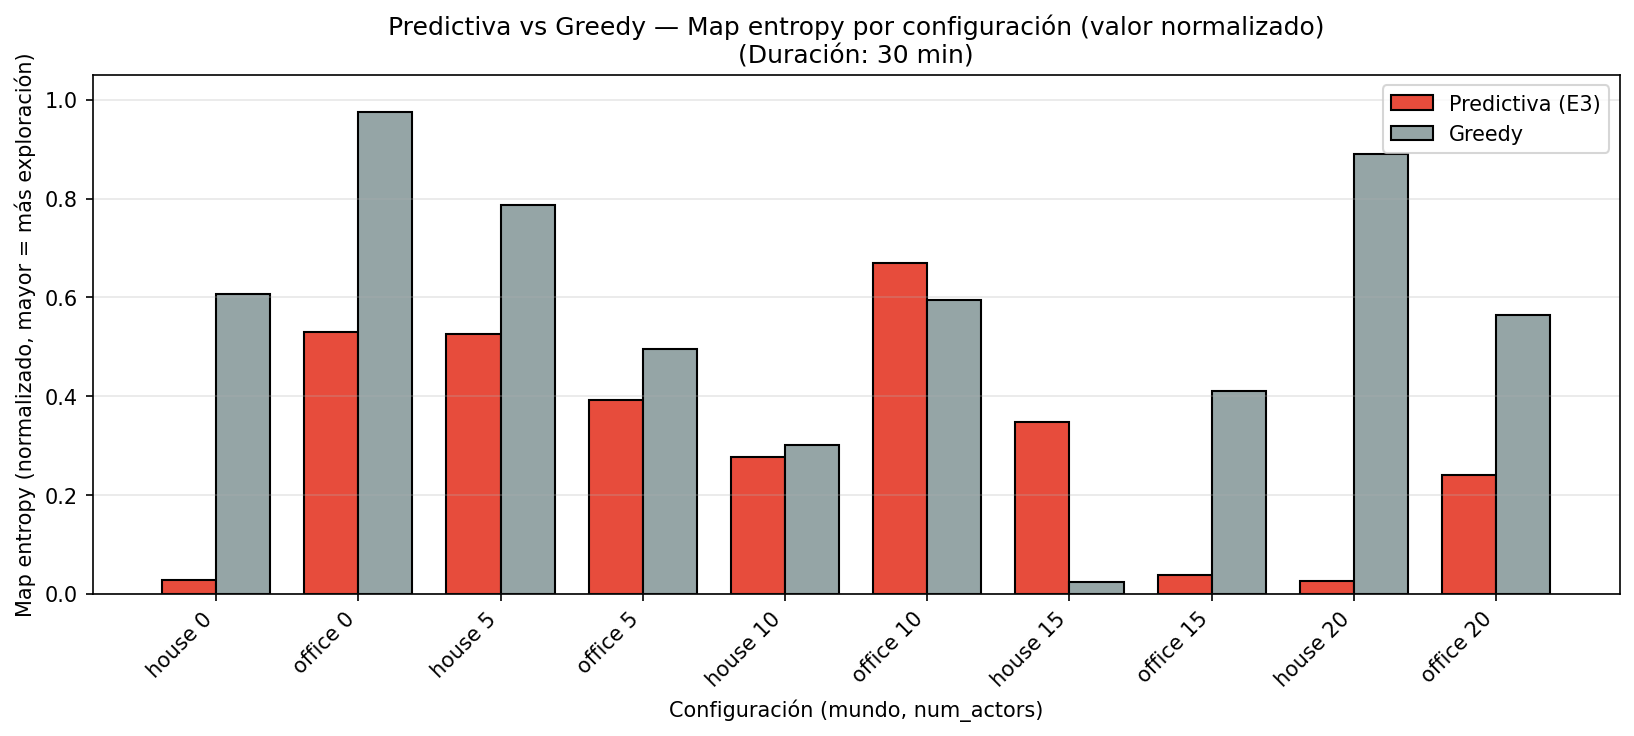
\includegraphics[width=0.85\textwidth]{figures/experiments/e3_vs_greedy_06_entropy_normalizado.png}
    \caption{Entropía del mapa normalizada por configuración. Valor normalizado mayor indica mayor exploración. Greedy supera a Predictiva en 8 de las 10 configuraciones.}
    \label{fig:e3_entropy}
\end{figure}

En entropía del mapa Greedy supera a la estrategia Predictiva en \textbf{8 de las 10} configuraciones. Predictiva únicamente supera a Greedy en office-10 ($+12\%$) y en house-15 ($+710\%$, caso particular con entropía muy baja de Greedy). Esta desventaja generalizada en exploración se atribuye al mayor costo computacional de la estrategia Predictiva, detallado en la Sección~\ref{sec:exp_e3_costo}.

La Tabla~\ref{tab:e3_frames} y la Figura~\ref{fig:e3_frames} presentan los resultados de frames procesados.

\begin{table}[htbp]
    \centering
    \caption{Frames totales procesados (valor final acumulado) por configuración: Predictiva vs Greedy. Valores en negrita indican la estrategia ganadora. Mayor es mejor.}
    \label{tab:e3_frames}
    \begin{tabular}{lrrr}
        \toprule
        \textbf{Configuración} & \textbf{Predictiva (mediana)} & \textbf{Greedy} & \textbf{\% dif.} \\
        \midrule
        house-0   & \textbf{620}  & 217  & $+186\%$ \\
        office-0  & \textbf{613}  & 555  & $+10\%$  \\
        house-5   & 449           & \textbf{577} & $-22\%$ \\
        office-5  & 523           & \textbf{648} & $-19\%$ \\
        house-10  & 419           & \textbf{454} & $-8\%$  \\
        office-10 & \textbf{638}  & 601  & $+6\%$   \\
        house-15  & 340           & \textbf{597} & $-43\%$ \\
        office-15 & 509           & \textbf{607} & $-16\%$ \\
        house-20  & \textbf{437}  & 265  & $+65\%$  \\
        office-20 & \textbf{596}  & 98   & $+508\%$ \\
        \bottomrule
    \end{tabular}
\end{table}

\begin{figure}[htbp]
    \centering
    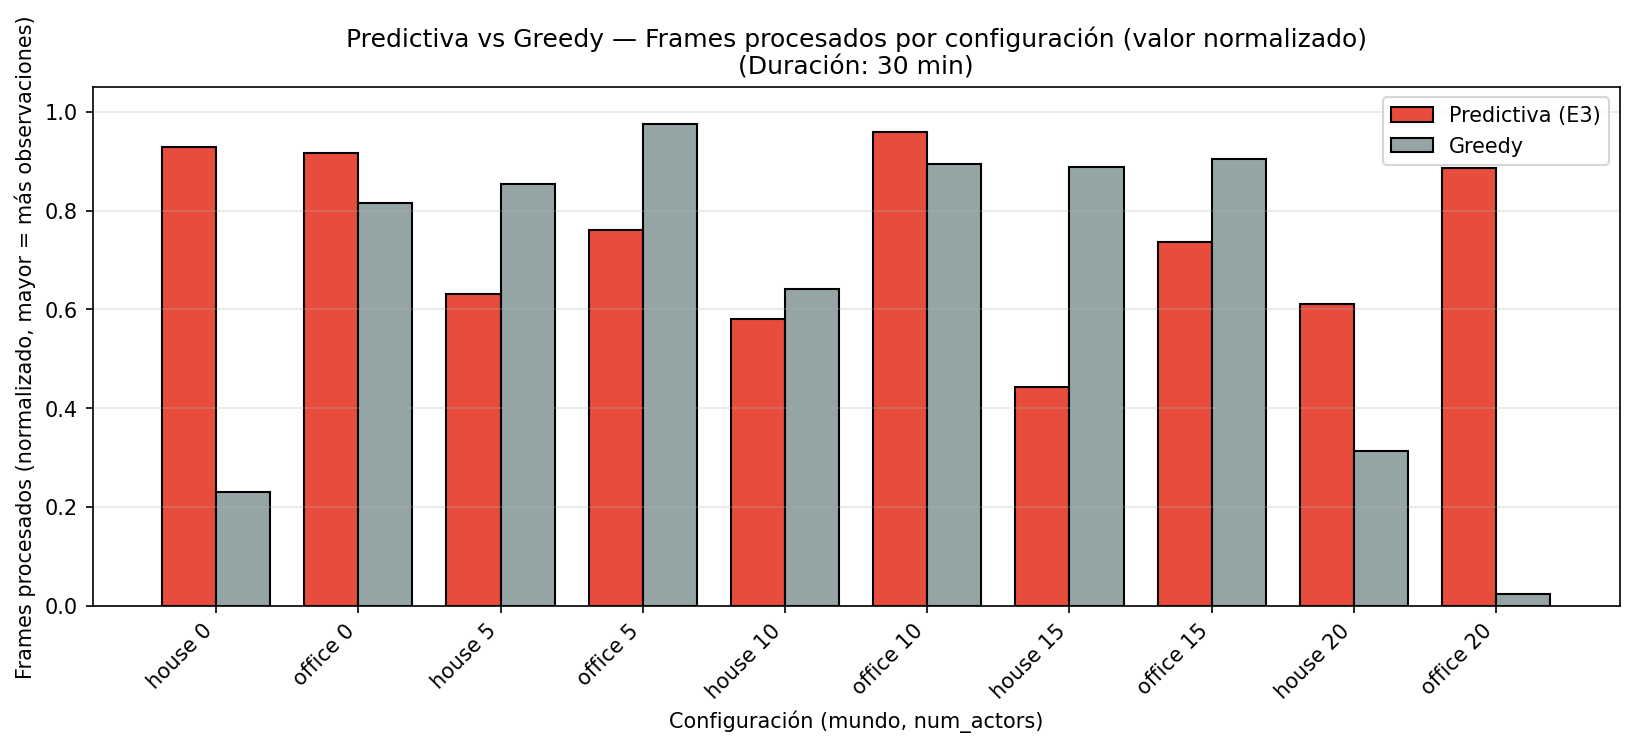
\includegraphics[width=0.85\textwidth]{figures/experiments/e3_vs_greedy_07_frames_normalizado.png}
    \caption{Frames procesados normalizados por configuración. Valor normalizado mayor indica mayor throughput del pipeline de visión. Predictiva supera a Greedy en 5 de las 10 configuraciones.}
    \label{fig:e3_frames}
\end{figure}

En frames procesados la estrategia Predictiva supera a Greedy en \textbf{5 de las 10} configuraciones. Las ventajas más marcadas se observan en house-0 ($+186\%$) y en office-20 ($+508\%$). En los casos con densidad intermedia de actores (house-5, office-5, house-10, house-15, office-15) Greedy procesa más frames, lo que es coherente con su menor tiempo de cómputo por decisión.

\subsection{Puntuación compuesta y análisis global}
\label{sec:exp_e3_score}

La Figura~\ref{fig:e3_score_config} presenta la puntuación compuesta calculada con la Ecuación~(\ref{eq:score}) para cada configuración, y la Figura~\ref{fig:e3_victorias} resume el recuento de victorias por métrica.

\begin{figure}[htbp]
    \centering
    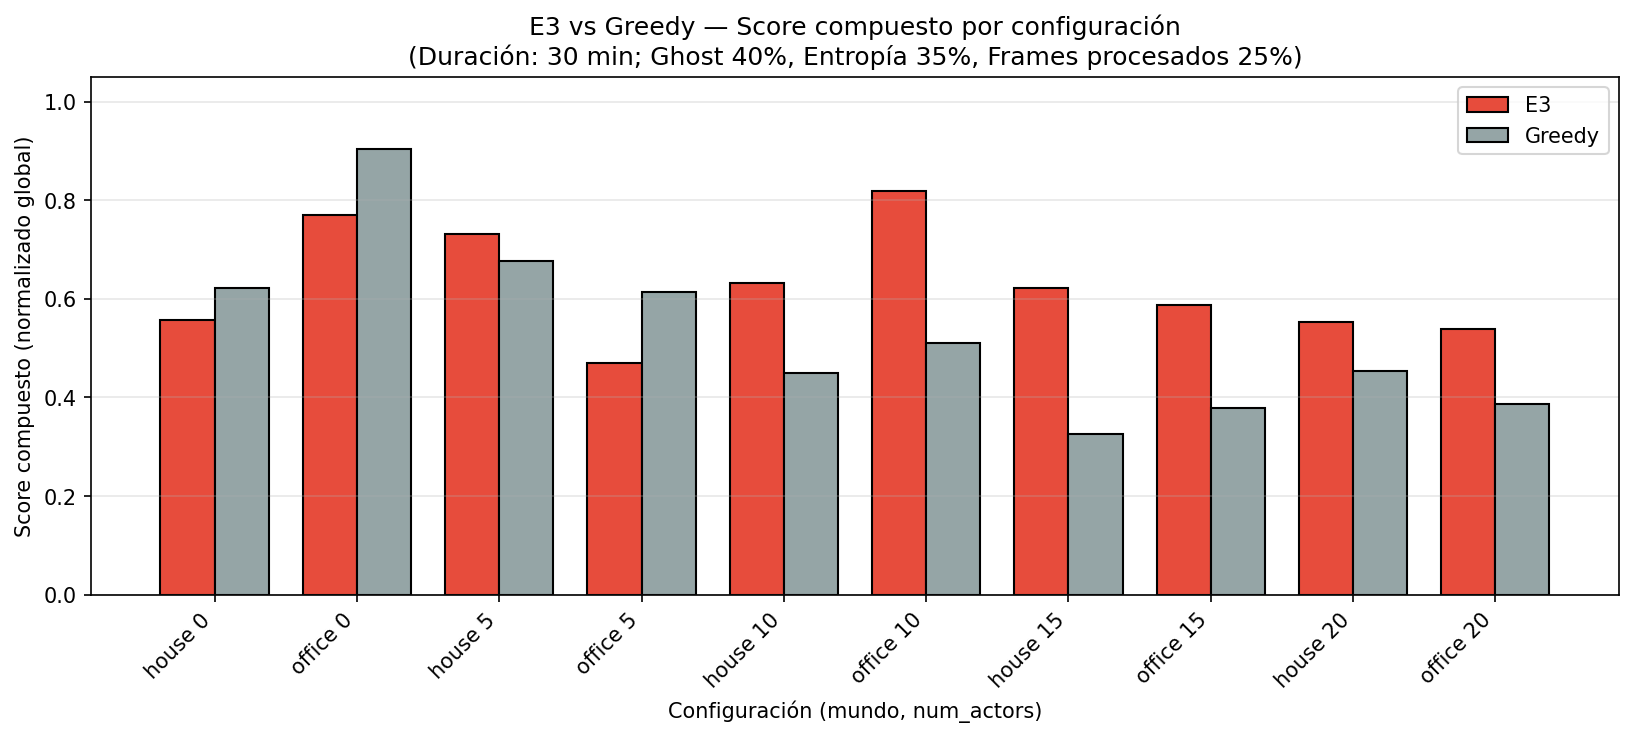
\includegraphics[width=0.85\textwidth]{figures/experiments/e3_vs_greedy_01_score_por_config.png}
    \caption{Puntuación compuesta por configuración (Predictiva vs Greedy). Pesos: celdas fantasma 40\%, entropía 35\%, frames 25\%. Predictiva supera a Greedy en 7 de las 10 configuraciones.}
    \label{fig:e3_score_config}
\end{figure}

\begin{figure}[htbp]
    \centering
    \begin{subfigure}[b]{0.55\textwidth}
        \centering
        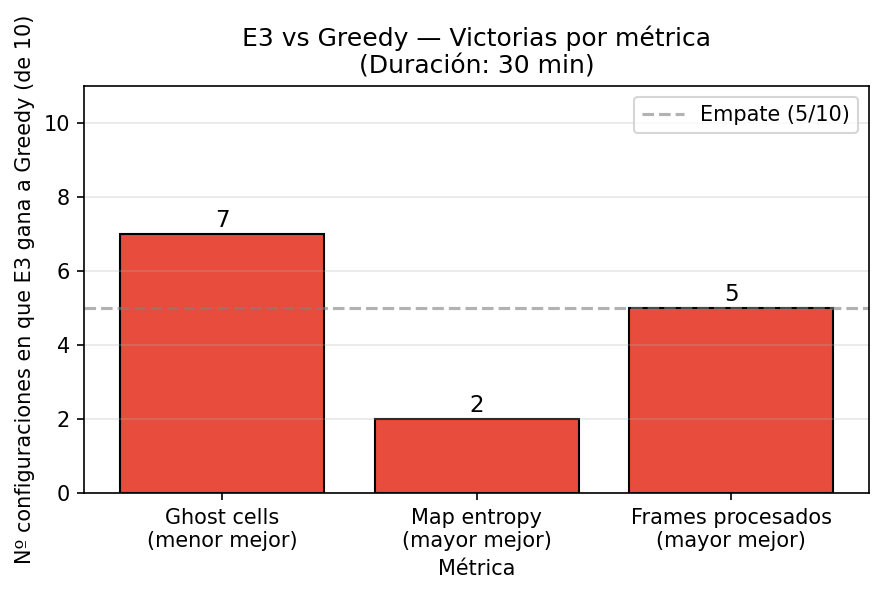
\includegraphics[width=\textwidth]{figures/experiments/e3_vs_greedy_03_victorias_por_metrica.png}
        \caption{Victorias por métrica individual.}
        \label{fig:e3_victorias_metrica}
    \end{subfigure}
    \hfill
    \begin{subfigure}[b]{0.40\textwidth}
        \centering
        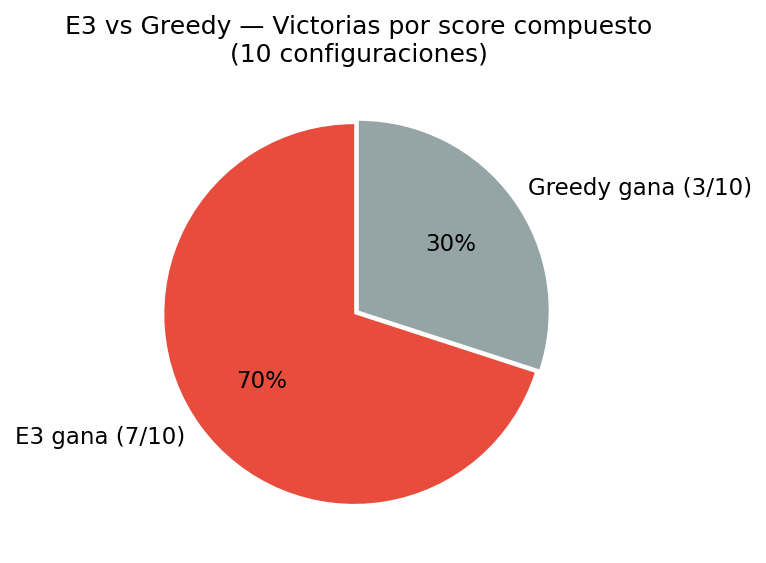
\includegraphics[width=\textwidth]{figures/experiments/e3_vs_greedy_04_torta_victorias_score.png}
        \caption{Victorias por puntuación compuesta.}
        \label{fig:e3_victorias_score}
    \end{subfigure}
    \caption{Resumen de victorias de la estrategia Predictiva frente a Greedy. Predictiva gana en 7/10 configuraciones por puntuación compuesta.}
    \label{fig:e3_victorias}
\end{figure}

Por puntuación compuesta, la estrategia Predictiva es la ganadora en \textbf{7 de las 10} configuraciones: TC023 (house-5), TC025 (house-10), TC026 (office-10), TC027 (house-15), TC028 (office-15), TC029 (house-20) y TC030 (office-20). En las tres configuraciones restantes (TC021, TC022, TC024, correspondientes a house-0, office-0 y office-5) Greedy obtiene mayor puntuación, en todos los casos sin actores o con densidad muy baja donde Predictiva no dispone de información dinámica relevante para guiar su planificación.

Aplicando el criterio de cuasi-empate ($S_{\text{Pred}} \geq 0{,}9 \cdot S_{\text{Greedy}}$), la estrategia Predictiva resulta competitiva o mejor en \textbf{7 de las 10} configuraciones. Este resultado indica que Predictiva no solo supera a la línea de base en la mayoría de los casos, sino que incluso en las configuraciones que no gana, la diferencia en puntuación compuesta es reducida en la mayor parte de ellas.

\subsection{Análisis por entorno}
\label{sec:exp_e3_entorno}

\textbf{Entorno house.} En celdas fantasma, Predictiva supera a Greedy en todas las configuraciones con actores (5, 10, 15 y 20) y únicamente pierde en el caso sin actores. En entropía, Predictiva supera a Greedy solo en house-15; en los demás casos Greedy explora más del mapa. En frames procesados, Predictiva supera a Greedy en house-0 y house-20. La puntuación compuesta es favorable a Predictiva en cuatro de las cinco configuraciones de house (TC023, TC025, TC027, TC029).

\textbf{Entorno office.} En celdas fantasma, Predictiva supera a Greedy en las configuraciones con 10, 15 y 20 actores, mientras que pierde con 0 y 5. En entropía, Predictiva supera a Greedy únicamente en office-10. En frames procesados, Predictiva supera a Greedy en office-0, office-10 y con una diferencia muy marcada en office-20 ($+508\%$). La puntuación compuesta favorece a Predictiva en TC026, TC028 y TC030 (office-10, office-15 y office-20).

En conjunto, los resultados revelan que el beneficio de la estrategia Predictiva se incrementa con la densidad de actores en ambos entornos. La ventaja en precisión de mapa (celdas fantasma) es robusta a partir de densidades de 5 actores en house y 10 actores en office. La ventaja en exploración (entropía) es menos frecuente, lo que se discute en la sección siguiente.

\subsection{Análisis del costo computacional}
\label{sec:exp_e3_costo}

La desventaja de la estrategia Predictiva en exploración (entropía del mapa) en los experimentos de 30 minutos motivó el planteamiento de la \textbf{hipótesis del costo computacional}: la menor exploración de Predictiva puede deberse en parte a la demora en el cálculo de la utilidad dinámica, que involucra la planificación de la ruta completa hacia cada frontera candidata, el cómputo del tiempo de viaje a cada punto de la ruta y la predicción de posiciones futuras de cada persona detectada. Esta demora reduce el tiempo efectivo de movimiento del robot por ciclo de decisión.

Para contrastar esta hipótesis, se ejecutaron dos experimentos de mayor duración (aproximadamente tres horas) con la configuración de mayor densidad de actores en cada entorno:

\begin{itemize}
    \item \textbf{VH001}: house-20, duración $\approx 2{,}99$ h.
    \item \textbf{VH002}: office-20, duración $\approx 2{,}99$ h.
\end{itemize}

La Figura~\ref{fig:e3_costo_evolucion} muestra la evolución temporal de la entropía del mapa y los frames procesados a lo largo de los experimentos extendidos. La Figura~\ref{fig:e3_costo_comparacion} compara los valores finales de los experimentos de 30 minutos con los de 3 horas.

\begin{figure}[htbp]
    \centering
    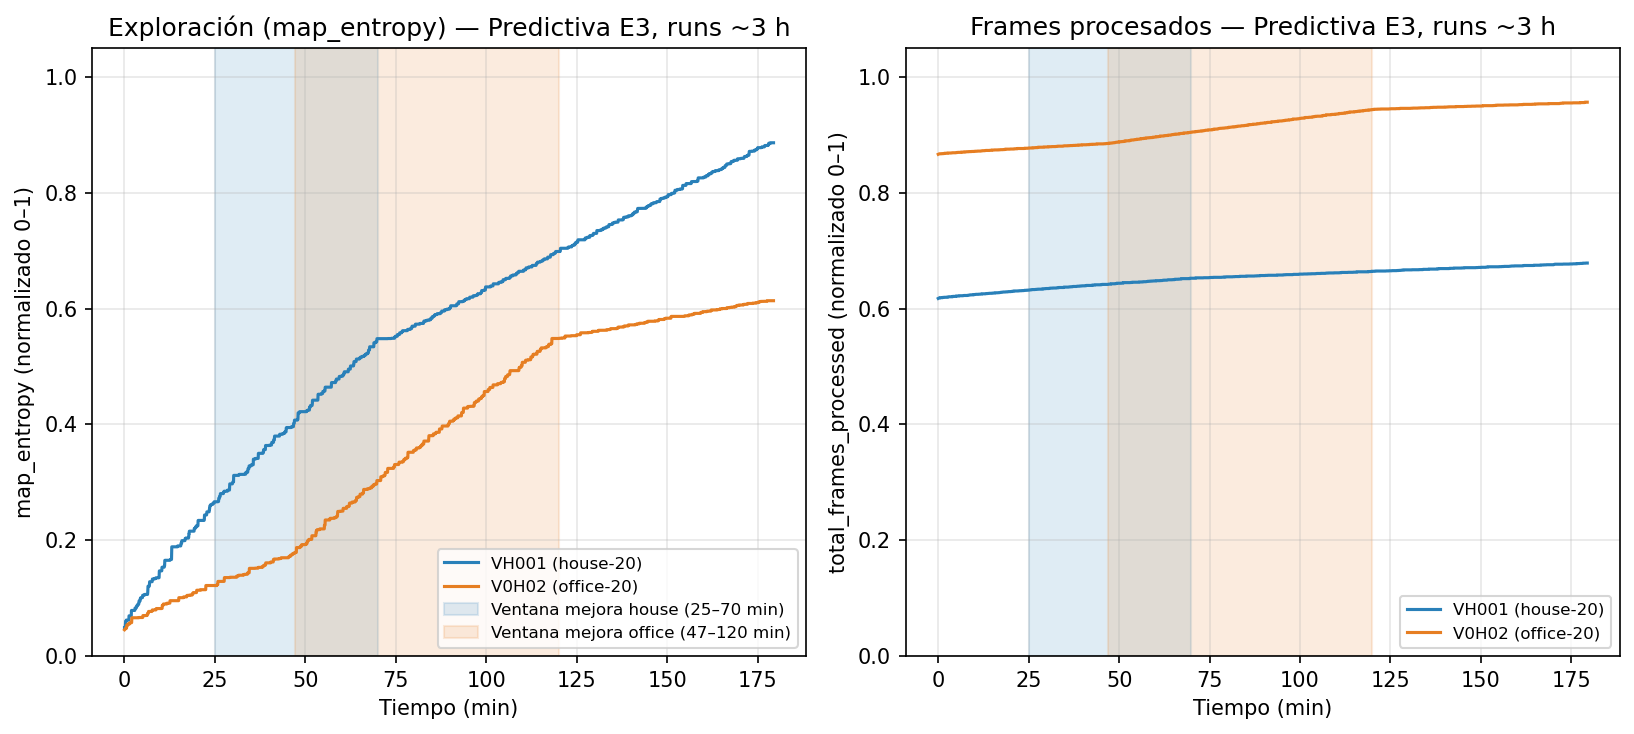
\includegraphics[width=0.90\textwidth]{figures/experiments/cost_hypothesis_01_evolution_time.png}
    \caption{Evolución temporal de la entropía del mapa y los frames procesados en los experimentos extendidos (VH001 y VH002, $\approx 3$ h). Se observa una ventana de crecimiento acelerado entre los 25--70 min en house y entre los 47 min y 2 h en office, seguida de una fase de mejora leve.}
    \label{fig:e3_costo_evolucion}
\end{figure}

\begin{figure}[htbp]
    \centering
    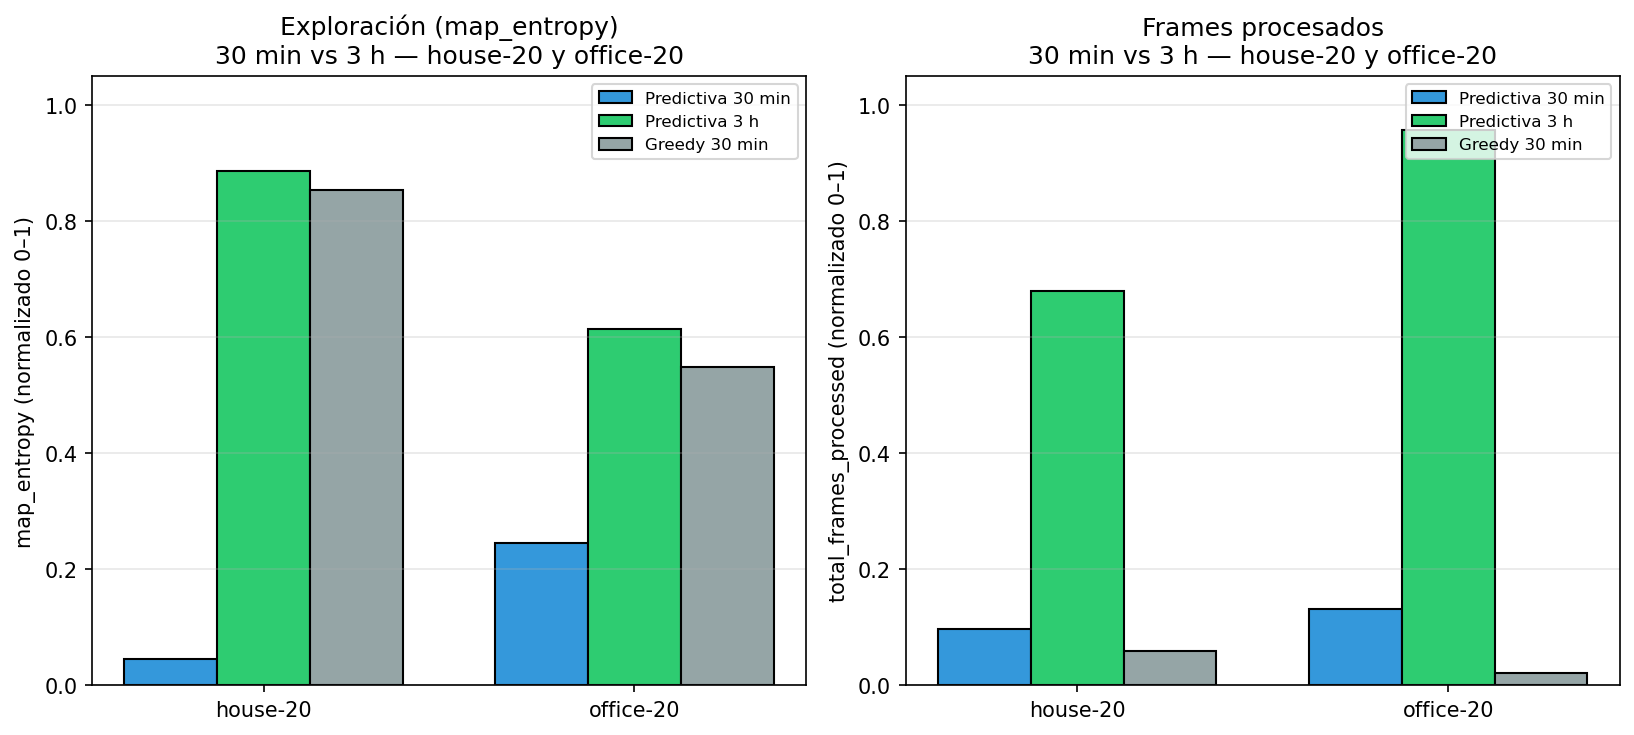
\includegraphics[width=0.85\textwidth]{figures/experiments/cost_hypothesis_02_comparison_30min_vs_3h.png}
    \caption{Comparación de métricas finales entre los experimentos de validación (30 min) y los experimentos extendidos ($\approx 3$ h) para las configuraciones house-20 y office-20. Se incluyen los valores de Greedy a 30 min como referencia.}
    \label{fig:e3_costo_comparacion}
\end{figure}

Los resultados de los experimentos extendidos se resumen a continuación:

\begin{itemize}
    \item \textbf{house-20 (VH001):} a 30 min, Predictiva registró 437 frames y entropía $9{,}83 \times 10^{-6}$. A 3 h, los valores alcanzaron 3054 frames y entropía $1{,}95 \times 10^{-4}$, superando ampliamente los valores de Greedy a 30 min (265 frames, $1{,}88 \times 10^{-4}$).
    \item \textbf{office-20 (VH002):} a 30 min, Predictiva registró 596 frames y entropía $5{,}41 \times 10^{-5}$. A 3 h, los valores alcanzaron 4304 frames y entropía $1{,}35 \times 10^{-4}$, superando también a Greedy a 30 min (98 frames, $1{,}21 \times 10^{-4}$).
\end{itemize}

Estos resultados apoyan la hipótesis: dado tiempo suficiente, la estrategia Predictiva recupera y supera la exploración de Greedy en ambos entornos. La ventana de crecimiento acelerado es distinta en cada entorno (25--70 min en house; 47 min--2 h en office), lo que sugiere que la dificultad de recuperación depende de la geometría del entorno y la complejidad de las rutas calculadas. Para que Predictiva exprese su potencial de exploración junto con su ventaja en precisión, se recomienda asignar al menos 1--2 horas de ejecución.

\subsection{Discusión}
\label{sec:exp_e3_discusion}

Los resultados permiten identificar tres aspectos centrales del comportamiento de la estrategia Predictiva:

\textbf{Precisión del mapa.} La predicción de interferencia es el mecanismo que explica la reducción de celdas fantasma. Al estimar qué personas cruzarán la ruta hacia cada frontera, AlfredZ evita o posterga las fronteras donde la presencia futura de personas generaría ocupaciones transitorias en el mapa. Este efecto es estructural: crece con la densidad de actores y es independiente del entorno, razón por la que se observa en house y office a partir de 5--10 actores. La estrategia Greedy, que selecciona únicamente por distancia, no dispone de este mecanismo y acumula celdas fantasma en proporción a la actividad dinámica del entorno.

\textbf{Exploración.} La desventaja de Predictiva en entropía del mapa en los experimentos de 30 minutos no obedece a decisiones subóptimas de exploración, sino principalmente al mayor costo computacional por ciclo de decisión. Los experimentos extendidos demuestran que, con tiempo suficiente, Predictiva alcanza y supera el nivel de exploración de Greedy. Este hallazgo sugiere que la comparación a 30 minutos subestima el potencial de la estrategia Predictiva en aplicaciones de mayor duración.

\textbf{Eficiencia.} El comportamiento de los frames procesados es heterogéneo: Predictiva supera a Greedy en las configuraciones sin actores y en las de mayor densidad, mientras que Greedy procesa más frames en densidades intermedias. Esta variabilidad refleja la interacción entre el costo computacional adicional de Predictiva y la reducción de interrupciones por colisión con personas que proporciona la predicción de interferencia.

En conjunto, los resultados \textbf{validan la estrategia Predictiva} como alternativa superior a Greedy cuando se prioriza la precisión del mapa o cuando el tiempo de exploración disponible es suficiente. La estrategia Greedy resulta preferible únicamente cuando se requiere maximizar la exploración en ventanas de tiempo cortas y la densidad de actores es baja o nula.
